\documentclass[12pt, letterpaper]{article}
\usepackage[utf8]{inputenc} % 用于输入编码设置
\usepackage{CJKutf8} %中文
\usepackage{graphicx} %图片包
\usepackage{xcolor} %字体颜色
\usepackage{caption} % 加载 caption 包 去掉Figure 1
\usepackage{amsmath} %数学包



\begin{document}
\begin{CJK*}{UTF8}{gbsn}%显示中文% gbsn 宋体
% gkai 楷体

\title{Zusammenfassung des OM}
\author{Jiaqi Wang} % 可以在此处添加作者名
\date{22.12.2024} % 此命令插入当前日期
\maketitle % 这个命令会插入标题、作者和日期
\pagenumbering{gobble} %隐藏页码

\vspace{5cm}

\section{Einführung} % 文章第一节,引言
\begin{itemize}
\item Definition von OM: Operations Management ist der Überbegriff für das Management von Produktions- und Dienstleistungsprozessen und
befasst sich maßgeblich mit \textbf{produktionswirtschaftlichen} und \textbf{logistischen Fragestellungen}

\item vier "rs" in der Logistik: mti dem \textbf{richtigen} Produkt, im \textbf{richtigen} Zustand, zur \textbf{richtigen} Zeit, am \textbf{richtigen} Ort

\end{itemize}


%%%%%%%%%%%%%%%%%%%%
\newpage
\pagenumbering{arabic}%显示页码

\section{Absatzplanung}

\begin{enumerate}
\item Referenzmodell OM:\\
1. Planungshorizont: Jahre bis Tage (Zeitachse)\\
2. Planungsprobleme: Absatzprognose, Absatzplanung\\
3. Planungsgegenstand: Absatzmengen nach Produktfamilie bis Endprodukt\\
4. Input: historische Nachfragendaten, Expertenwissen\\
5. Output: Absatzmengen

\item Elemente der Absatzplannung:\\
1. Absatzprognose: ist eine Grundeinschätzung zukünftigen Bedarfs basierend
auf statistischen Methoden\\
2. Absatzplanung: ist eine auf der Prognose beruhende Bedarfsschätzung,
ergänzt um Expertenwissen und im Konsens abgestimmt\\

\item 1. Ordnung: gleichbleibende Nachfrage\\
\textbf{konstantes} Nachfrageniveau\\

\begin{figure}[h!]
  \centering % 居中显示图片
  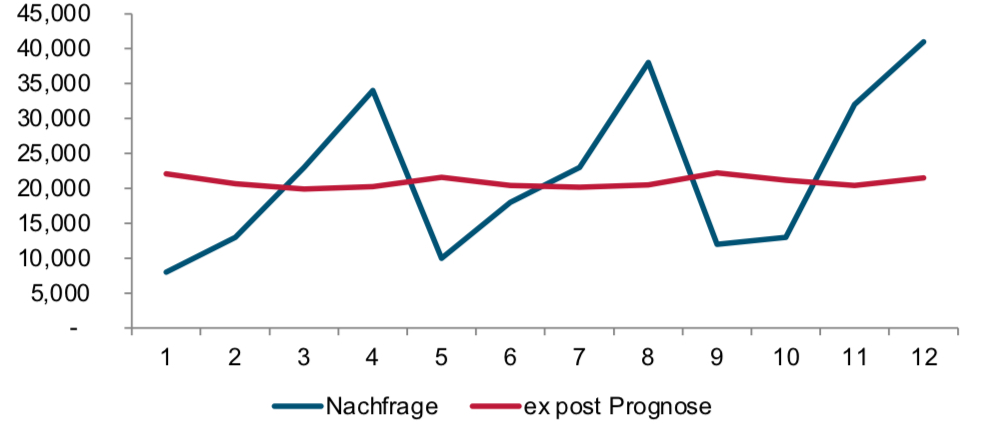
\includegraphics[width=0.5\linewidth]{UE11.jpg}\\[5cm]
\end{figure}

\item 2. Ordnung: trendförmig ansteigende Nachfrage\\
Niveau der Zeitreihe steigt \textbf{linear}\\

\begin{figure}[h!]
  \centering % 居中显示图片
  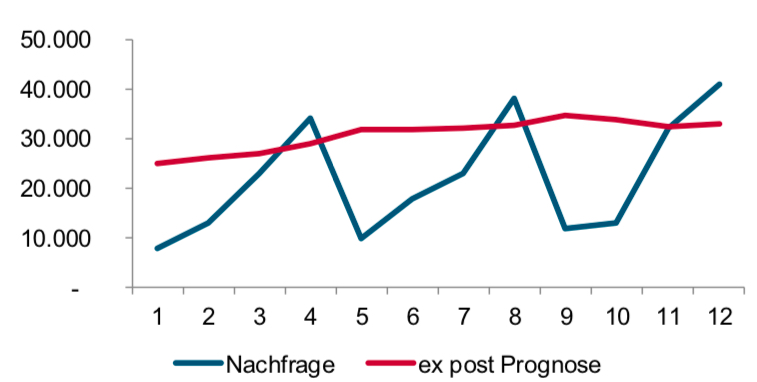
\includegraphics[width=0.5\linewidth]{UE12.jpg}
\end{figure}

\item 3. Ordnung: saisonal schwankende Nachfrage\\
Niveau der Zeitreihe steigt \textbf{linear}\\

\begin{figure}[h!]
  \centering % 居中显示图片
  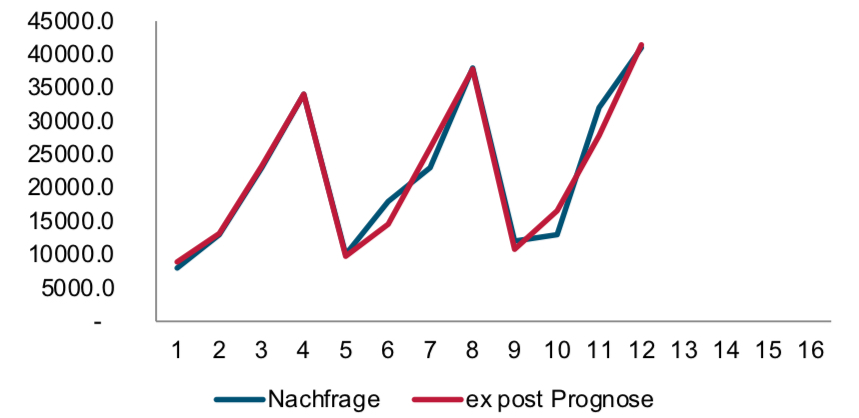
\includegraphics[width=0.5\linewidth]{UE13.jpg}
\end{figure}

\item Type von Prognosenfehler:
\begin{itemize}
\item Mittlerer Fehler nach n Perioden
\item Mittlerer absoluter Fehler nach n Perioden
\item Mittlerer prozentualer Fehler
\item Mittlerer absoluter prozentualer Fehler
\end{itemize}


\end{enumerate}

%%%%%%%%%%%%%%%%%%%%
\newpage

\section{Beschaffungs- und Distributionslogistik}
\subsection{Beschaffungsstrategie}
\begin{itemize}
\item Klassifizierung der Beschaffungsartikel\\
\begin{figure}[h!]
  \centering % 居中显示图片
  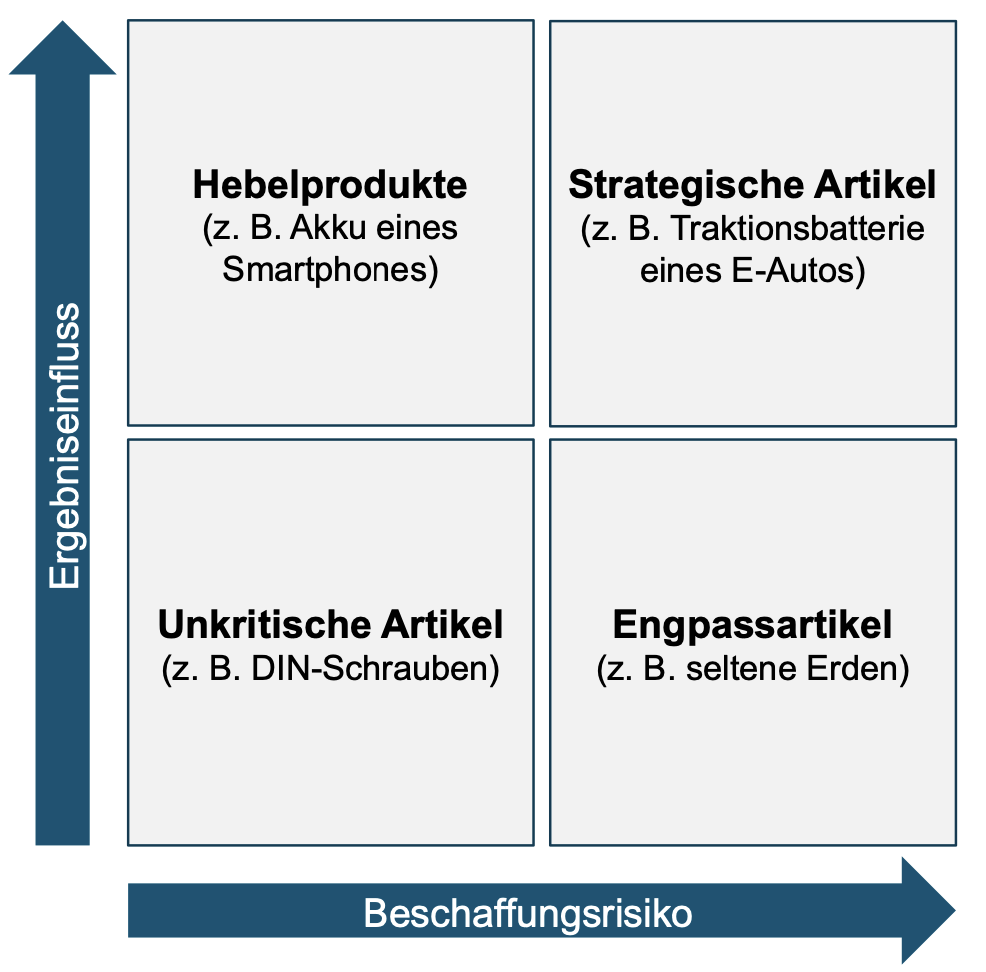
\includegraphics[width=0.6\linewidth]{VL31.png}\\
   \caption*{Beschaffungsrisiko: 供应商延迟交货, 原材料价格波动, 供应链中断\\
   Ergebniseinfluss: 任何可影响公司整体业绩的因素}
\end{figure}
\end{itemize}

\subsection{Beschaffungsstruktur}
\begin{itemize}
\item Global Sourcing vs. Regional Sourcing:\\
Nutzung weltweiter oder regionaler Beschaffungsstrukturen\\
\item Single vs. Multiple Sourcing\\
Nutzung eines oder mehrerer Lieferanten für die gleichen Teile\\
\item Modular vs. Unit Sourcing\\
Beziehung einer Baugruppe auf Bauteil- oder Baugruppenebene
\end{itemize}

\subsection{Bereitstellungskonzepte}
\begin{itemize}
\item Auftragsbezogene Beschaffung: (有了订单 再买货物)\\
\begin{figure}[h!]
  \centering % 居中显示图片
  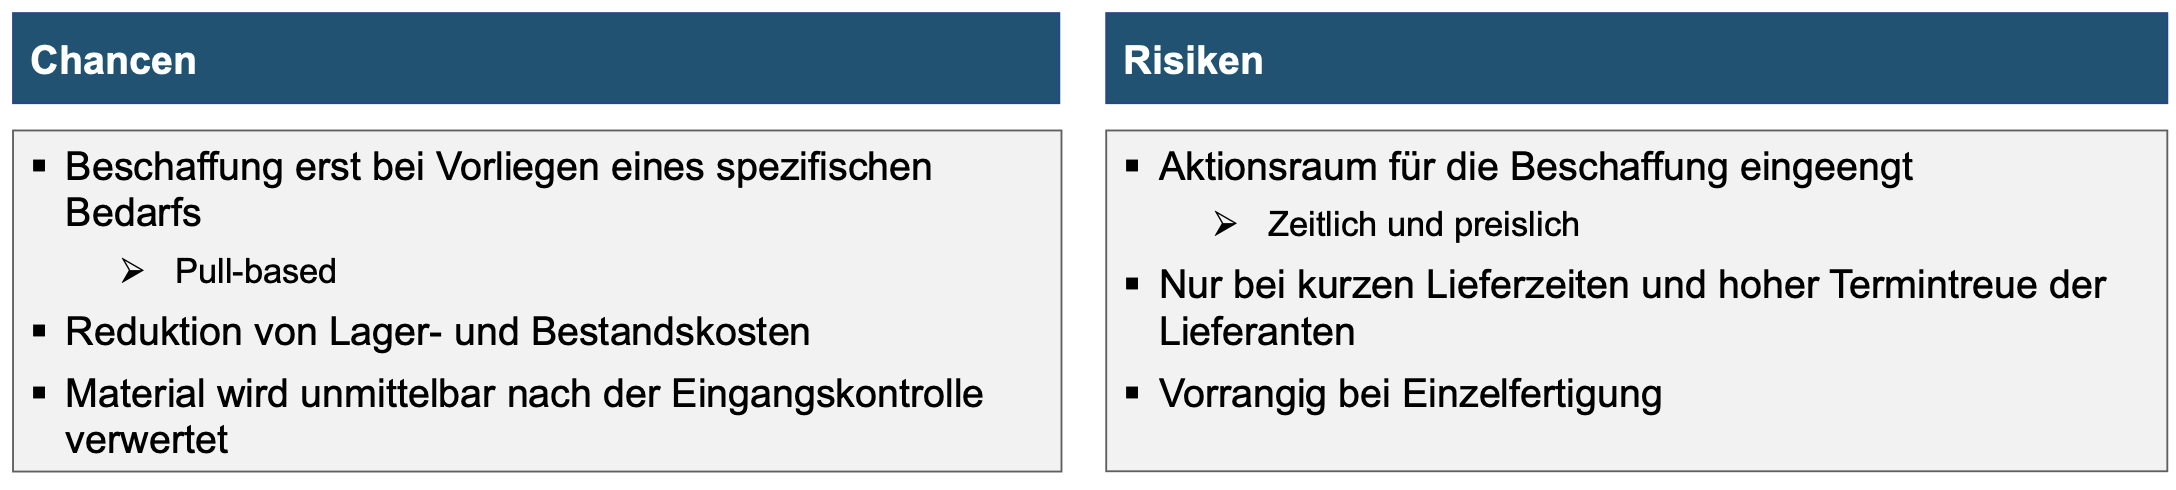
\includegraphics[width=0.7\linewidth]{VL32.png}\\
\end{figure}
Nachteil: \textcolor{red}{Hohe Unsicherheit}

\item Vorratsbeschaffung: (积累库存)\\
\begin{figure}[h!]
  \centering % 居中显示图片
  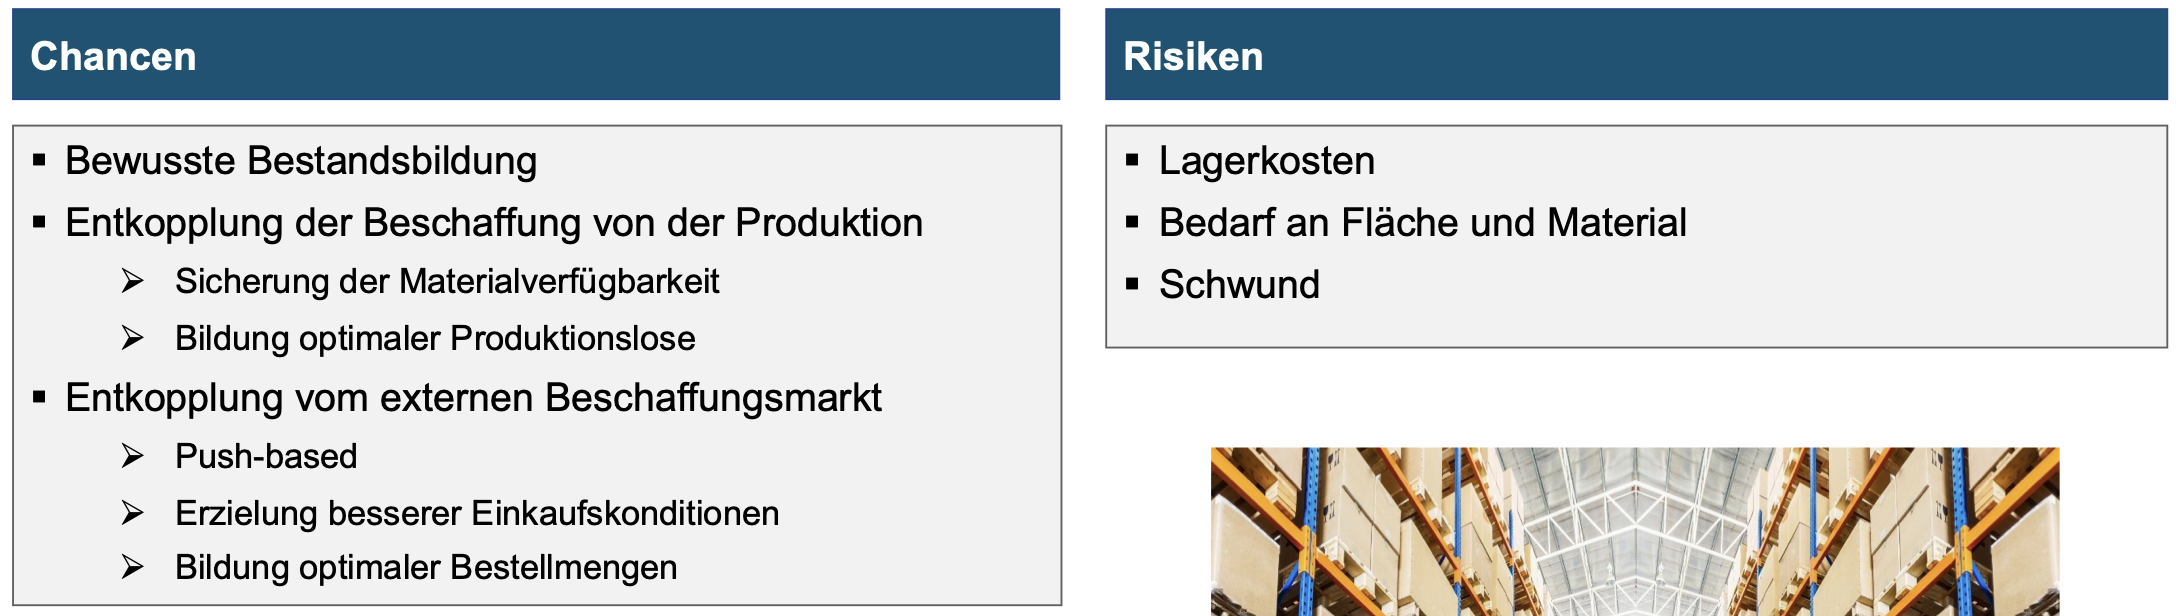
\includegraphics[width=0.7\linewidth]{VL33.png}\\
\end{figure}
Nachteil: \textcolor{red}{Hohe Lagerkosten}

\item Just In Time \& Just In Sequence\\
根据上述两个方法 引入的改良手段\\
Ziel: \textcolor{blue}{Möglichst nachfragegenaue Produktion und Beschaffung}


\item Produktionssynchrone Beschaffung: (边生产边买)\\
\begin{figure}[h!]
  \centering % 居中显示图片
  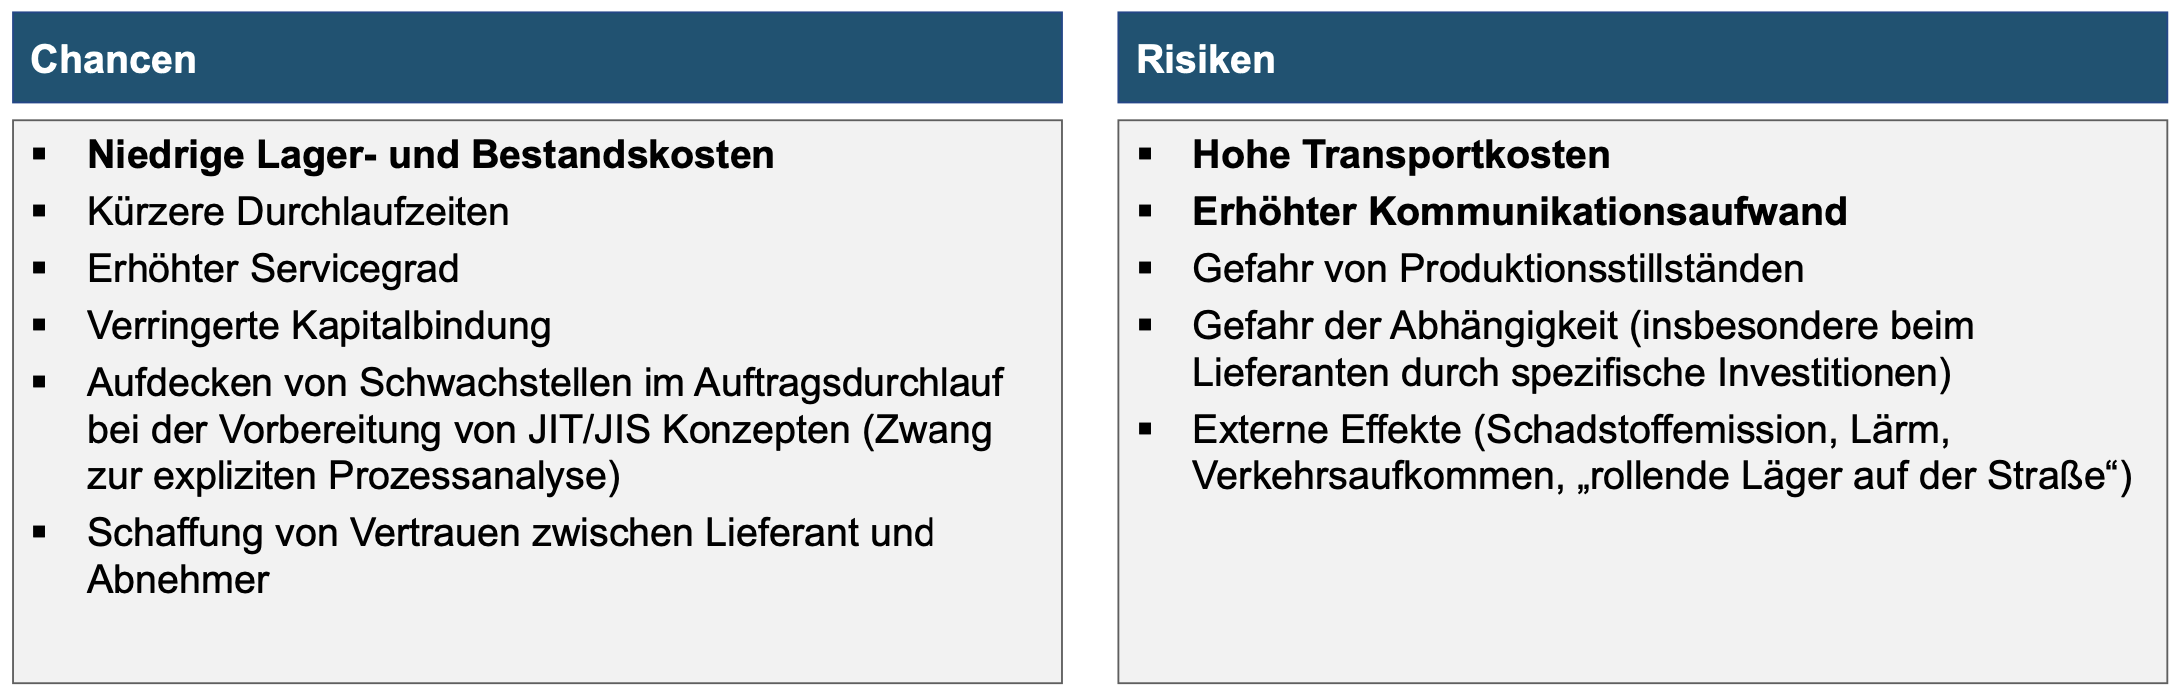
\includegraphics[width=0.7\linewidth]{VL34.png}\\
\end{figure}

\newpage
\item ABC-Analyse:\\
根据产品价值进行分类\\ 
专注于: Planungsaktivität \& Optimierungsbemühung

\begin{figure}[h!]
  \centering % 居中显示图片
  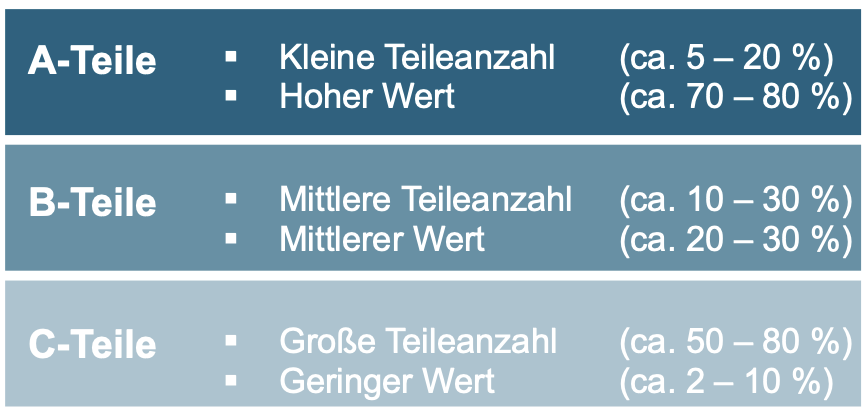
\includegraphics[width=0.4\linewidth]{VL35.png}\\
\end{figure}

\item XYZ-Analyse:\\
根据计划\&预测Sicherheit进行分类\\
也就是产品的  hohe, mittlere und schlechte Vorhersagegenauigkeit
\begin{figure}[h!]
  \centering % 居中显示图片
  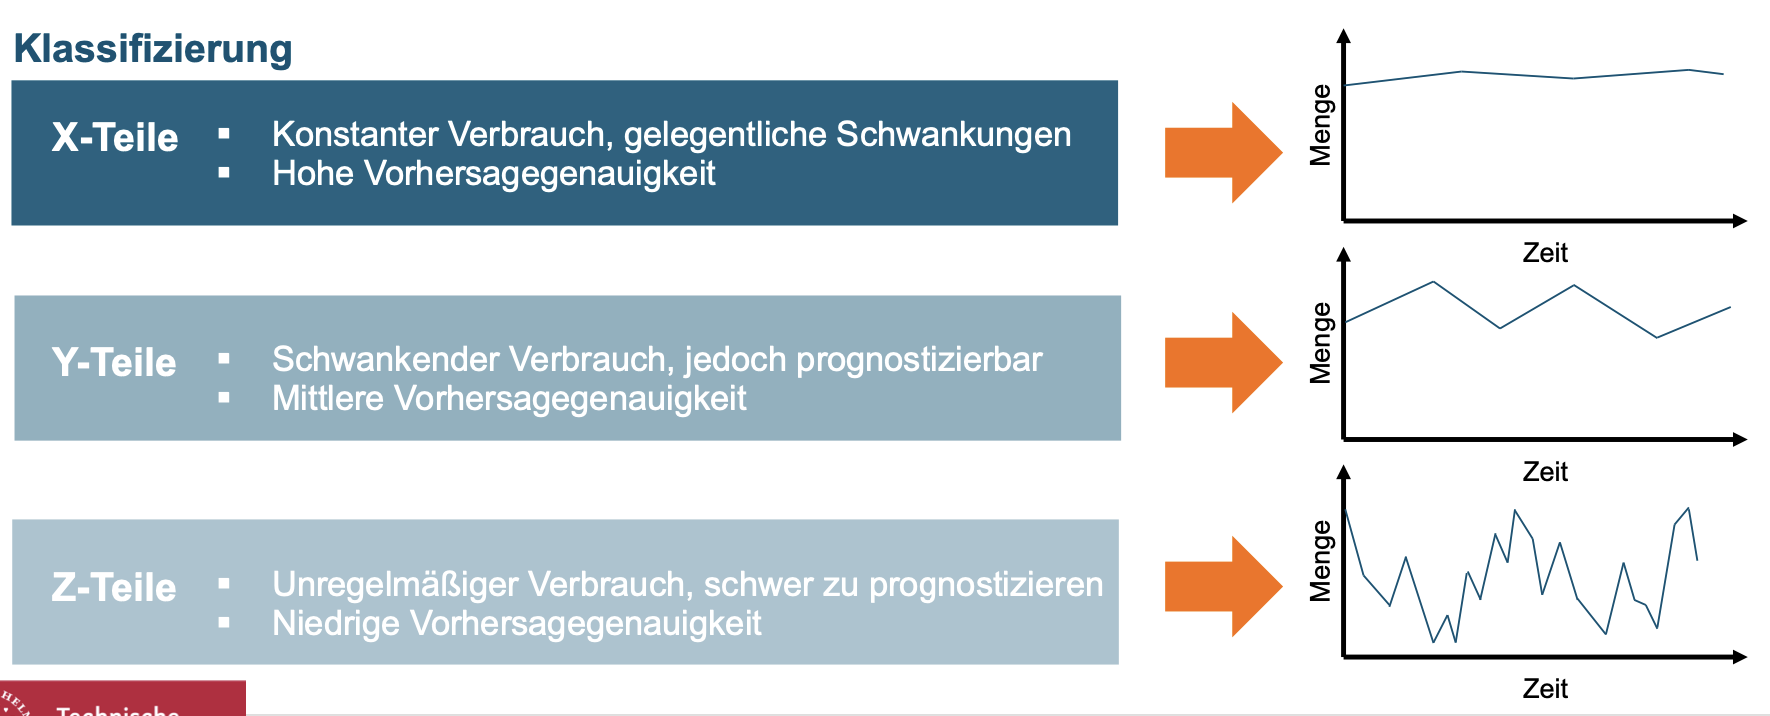
\includegraphics[width=0.6\linewidth]{VL36.png}\\
\end{figure}

\end{itemize}

\subsection{Distributionsstrategie}
\begin{itemize}
\item Werkslager 工厂仓库\\ 
nähe von Produktionsstätte

\item Zentrallager 中央仓库\\
Hoher Automatisierungsgrad und moderne Lagertechniken

\item Regionallager 区域仓库\\
Puffer zwischen Produktion und Absatzmarkt

\item Auslieferungslager 分发仓库\\
Dezentrale Ansiedlung im gesamten Verkaufsgebiet\\

\item vertikale \& horizontale Distributionsstruktur:\\[1mm]
vertikal: Anzahl der Lagerstufen\\[1mm]
horizontal: Anzahl der Läger pro Stufe
\item zentrale vs dezentrale Lagerhaltung\\[1mm]
zentral: 产品组合广泛,运输时间长,贵重物品,一个供货商,少量大客户\\[1mm]
dezentral: 产品组合单一,运输快,产品便宜,多个供货商,许多小客户\\
\end{itemize}

\newpage
\section{Netzwerkplanung}
\subsection{Modelle zur Standortplanung}
Ziel: \textcolor{blue}{Transformation einer qualitativen Bewertung verschiedener sich ausschließender Handlungsalternativen in eine einheitliche quantitative Nutzenskala}\\[1mm]
将各种互斥行动方案的定性评估转化为统一的定量效益尺度

\subsection{Standortplanung in Netzen}

\begin{itemize}
\item Warehouse Location Probleme (仓库选址问题)\\[1mm]
Ziel: Bestimmung eines oder mehrerer Standorte (und Transportmengen), so dass die \textcolor{blue}{Summe aus Fixkosten, variablen Betriebskosten und Transportkosten unter der Restriktion eines definierten Servicegrades minimiert wird}\\[1mm]
确定一个或多个位置(及运输量),以便在定义的服务等级的限制下,将固定成本、可变运营成本和运输\textcolor{red}{\textbf{成本的总和最小化}}

\item Funktion

\begin{flushleft}
dreistufiges kapazitiertes WLP:
\end{flushleft}

 \begin{itemize}
 \item  ZF: $Min Z =   \sum_{h=1}^{H} \sum_{i=1}^{I} \textcolor{red}{ \bar{c}_{hi} \cdot \bar{x}_{hi}} +
  \sum_{i=1}^{I} \sum_{j=1}^{J} \textcolor{blue}{c_{ij} \cdot x_{ij}} + 
  \sum_{i=1}^{I} \textcolor{green}{ f_i \cdot y_i}$

 
\begin{center}
\textcolor{red}{生产地 $\rightarrow$ 仓库} + \textcolor{blue}{仓库 $\rightarrow$ 客户} +  \textcolor{green}{仓库Fix}
\end{center}

\item 生产地容量限制: $\sum_{i=1}^{I}\bar{x}_{hi}\leq \bar{a}_h$\\
$\bar{a}_h$ 生产地容量

\item h到i的数量=i到j的数量: $\sum_{h=1}^{H}\bar{x}_{hi} - 
\sum_{j=1}^{J} x_{ij}$

\item 给客户的数量小于仓库极限: $\sum_{j=1}^{J}x_{ij} \leq b_i \cdot y_i$\\
$b_i$ 仓库容量 \ $y_i$ 0/1

\end{itemize}

\begin{flushleft}
zweistufiges kapazitiertes WLP: 将$\bar{x}$阉割掉
\end{flushleft}

\end{itemize}





%%%%%%%%%%%%
\newpage
\section{Produktionssegmentierung}
\subsection{Einführung}
Produktionssegment: Subsystem des Produktionsbereichs, welches eindeutig einem Organisationstyp zugeordnet
werden kann\\[1mm]
生产领域的子系统,可以明确地归属于一个组织类型。


\subsection{Layoutplanung in der Werkstattproduktion}
\begin{itemize}
\item Planungsprobleme in Abhängigkeit der Aggregationsebene(聚合级别)

\begin{enumerate}
\item Hohe Aggregationsebene: 确定厂的位置\\
\textcolor{purple}{Festlegung innerbetrieblicher Standorte} für Produktionssegmente
\item Niedrigere Aggregationsebene: 确定车间的位置\\
\textcolor{purple}{Festlegung von Standorten} innerhalb der einzelnen Produktionssegmente, z. B. Anordnung von Arbeitsplätzen im
Rahmen der Werkstattproduktion
\end{enumerate}


\item Planungsaufgaben

\begin{enumerate}
\item Neugestaltung: 第一次Layout空厂房\\
Erstmalige Bestimmung von Standorten für alle Produktionssegmente in einer leeren Fabrikhalle

\item Umstellung: 改变结构\\
Veränderung der Struktur des Materialflusses zwischen einzelnen Ressourcengruppen

\item Erweitung: 放置额外的生产部门\\
Platzierung eines zusätzlichen Produktionssegmentes
\end{enumerate}

\newpage

\item Funktion
\begin{itemize}

\item  ZF: $Min Z =   \sum_{ijkl}^{IJKL} 
\textcolor{red}{c} 
 \cdot \textcolor{blue}{x_{ij}}
 \cdot \textcolor{blue}{x_{kl}}
  \cdot \textcolor{green}{d_{jl}}
   \cdot \textcolor{purple}{t_{ik}}\ \  \   \underline{ nicht linear }$ 
   

\textcolor{red}{Kostensatz}\\
\textcolor{blue}{Maschine i/k 是否可放入Platz j/l \ 答案1/0}\\
\textcolor{green}{Differenz Platz d 和 j}\\
\textcolor{purple}{Transportmenge 机器i 和 k}
   
 \item Platz限制: $\sum_{i=1}^{I} x_{ij} \leq 1$
 \item 机器限制: $\sum_{i=1}^{I} x_{ij} = 1$\\[5mm]
 
\end{itemize}

\end{itemize}


\subsection{Assembly Line Balancing in der Fließproduktion}
根据产品数量 区分流水线种类
\begin{itemize}
\item Einprodukt-Fließproduktion (SALBP) 单品种物品流水线\\[1mm]
\textcolor{blue}{Produktion eines homogenen Produkts} mit hoher Qualität\\[1mm]
\textcolor{red}{Arbeitsinhalt konstant}

\item Mehrprodukt-Fließproduktion 多品种物品流水线\\[1mm]
\textcolor{blue}{Herstellung verschiedener Produkte} auf derselben Montagelinie

\item Multivarianten-Fließproduktion (MALBP) 多变量流水线\\[1mm]
\textcolor{blue}{Produktion verschiedener Varianten} auf derselben Montagelinie\\

\item Funktion 

\begin{itemize}
\item Taktzeit $c = \frac{3600 Sekunden}{Anzahl der Mengen}$ 
\item Station数量 $\lceil \frac{\sum \tau}{c} \rceil$
\end{itemize}

\newpage


\item 根据ZF区分SALBP \textbf{\textcolor{red}{Klausur Frage}}\\[1mm]
\begin{figure}[h!]
  \centering % 居中显示图片
  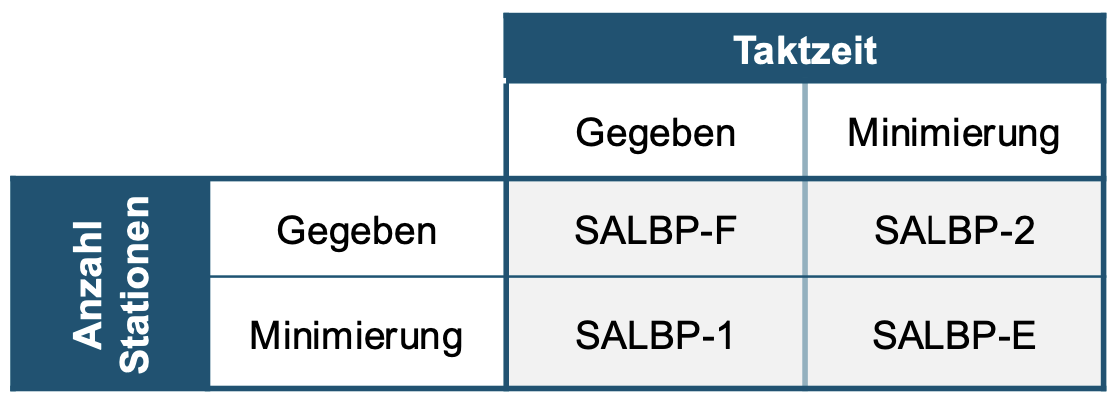
\includegraphics[width=0.4\linewidth]{VL51.png}
  \caption*{F:Machbarkeit, E:Effizient} % 为图片添加说明文字 *去掉Figure 1
\end{figure}
 
SALBP-1: Minimierung Anzahl, Taktzeit gegeben\\[1mm]
SALBP-2: Anzahl gegeben, Minimierung Taktzeit\\[1mm]
SALBP-F: beide gegeben \textcolor{blue}{所以牛逼}\\[1mm]
SALBP-E: beide Minimierung \textcolor{blue}{所以高效}

\end{itemize}


\newpage



%%%%%%%%%%%%%

\newpage
\section{Produktionsprogrammplanung}
\subsection{Beschäftigungsglättung}

\begin{itemize}
\item Modell AGGRPLAN\\
aggregierte Gesamtplanung 整体聚合规划\\
Ergebnis: Bestimmung der Produktionsmengen, eingesetzten Zusatzkapazitäten und Lagerbestände\\
Ziel: Minimierung der Kosten, Lagerkosten, Zusatzkapazitätskosten 


\item Funktion
\begin{itemize}

\item  ZF: $Min Z =   \sum_{kt}^{KT} 
\textcolor{red}{l_k \cdot L_{kt}} +
\sum_{t}^{T} \textcolor{blue}{u_t \cdot U_t}$ 
   

\textcolor{red}{Lagerkostensatz $\cdot$ Lagerbestand}\\
\textcolor{blue}{personeller \textcolor{purple}{\textbf{额外}}存储(Bezugkosten, Mehrkosten...)}

\item Bilanz: $X_{kt} + L_{k,t-1} - d_{kt} = L_{kt}$\\
该周期生产数+上周期剩余-卖出=该周期剩余

\item 技术限制: $\sum_{k=1}^{K}b_k \cdot X_{kt} \leq C^{max}_t$\\
$b_k$ 一单位造成的技术负载

\item 人员限制: $\sum_{k=1}^{K}a_k \cdot X_{kt} \leq N^{max}_t + \textcolor{purple}{U_t}$\\
$a_k$ 一单位造成的技术负载\\
最大personell 负载\ + \ personell\textcolor{purple}{\textbf{额外}}负载

\end{itemize}


\end{itemize}

\subsection{Kapazitierte Hauptproduktionsprogrammplanung}
\begin{itemize}
\item Modell HPPLAN\\
kapazitierte Hauptproduktionsprogrammplanung\\
Ergebnis \& Ziel 同上

\item 二者区别
\begin{enumerate}
\item AGGRPLAN 确定总体\\
\textcolor{blue}{aggregierte Sicht}: Nachfrageprognosen, Kapazitäten

\item HPPLAN 确定细节\\
\textcolor{blue}{detaillierte Sicht}: Nachfrageprognosen, Kapazitäten
\end{enumerate}

\item Funktion\\
几乎一样


\end{itemize}






%%%%%%%%%%%%%%%

\newpage
\section{Bestandsmanagement}
Bestandsmanagement beschäftigt sich mit der Betrachtung aller im Unternehmen vorhandenen Lagerbestände mit dem Ziel, \textcolor{blue}{die Kapitalbindung zu senken und eine größere Kapitalumschlagshäufigkeit} im Unternehmen zu erzielen\\[1mm]
库存管理涉及对公司内所有现有库存的审视,目的是降低资本占用,并在公司内实现更高的资本周转率\\

\begin{figure}[h!]
  \centering % 居中显示图片
  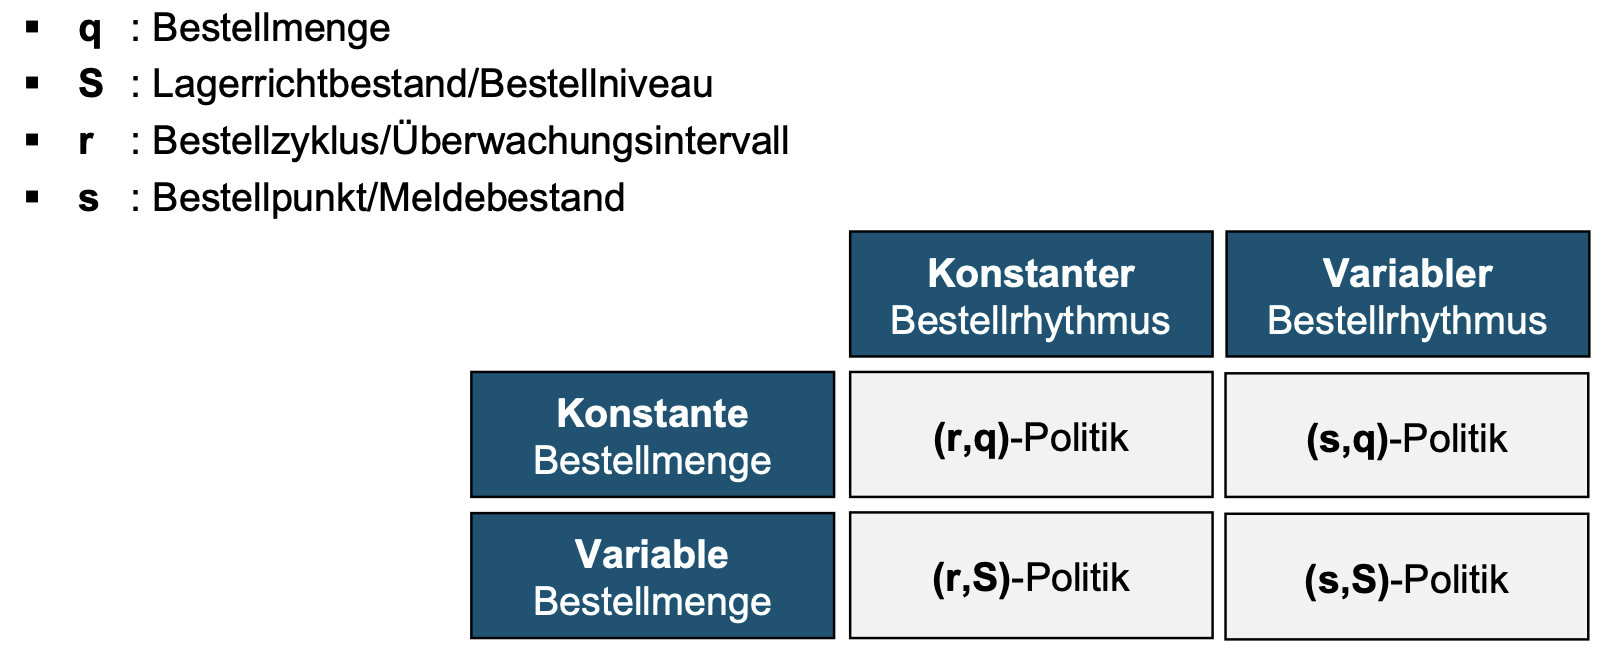
\includegraphics[width=0.8\linewidth]{VL71.png}
\end{figure}

\begin{itemize}

\item Leistungskennzahlen:
\begin{enumerate}

\item $\alpha$-ServiceGrad: Ereignisorientierte Kennzahl\\
Gibt die Wahrscheinlichkeit dafür an, dass die in einer Periode im Lager eintreffende Nachfrage vollständig und unverzüglich gedeckt werden kann

\begin{center}
$\alpha=P\leq S$
\end{center}

\item $\beta$-ServiceGrad: Ereignisorientierte Kennzahl\\
Gibt den zu erwartenden Anteil der sofort belieferten Nachfragemenge an der Gesamtnachfragemenge in einer Periode an
\begin{center}
$\beta=1- \frac{E\{Fehlmenge\ pro\ Periode\}}{E\{Nachfrage\}}$
\end{center}


\end{enumerate}


\end{itemize}


\newpage
\subsection{s,q-Politik}

\begin{itemize}
\item Begriff\\
variabler Bestellrhythmus bei konstanter Bestellmenge\\
\textcolor{red}{\textbf{计算订购时间点 s}}

\item Funktion

\begin{enumerate}

\item ZF:
\begin{center}
$Min z = s$\\
计算订购时间点 = 时间期望+Sicherheitsbestand\\
$s=E\{Y\}+SB=\mu_Y + SB$ \\
\end{center}

\item u.d.N.\\
\begin{center}
$E\{F_Y(s)\} \leq (1-\textcolor{purple}{\beta}) \cdot q_{opt}$\\
再补货时间内缺货量的期望 $\leq$非\textcolor{purple}{完成度}$\cdot$理想数
\end{center}


\item u.d.N. 辅助公式
\begin{center}
$E\{F_Y(s)\} = E\{F_U(v)\} \cdot \sigma_Y$\\
=安全系数v期望 $\cdot$ Standardabweichung
\end{center}

\item 辅助公式
\begin{center}
$\mu_Y = \mu_D \cdot L$\\
$\sigma_Y = \sigma_D \cdot \sqrt{L}$
\end{center}



\item optimale Bestallmenge(EOQ) \\
\begin{center}
$q_{opt} = \sqrt{\frac{2 \cdot D \cdot K_{bf}}{K_L}}$\\
\end{center}
D Nachfrage = $\mu_D$ Mittelwert\\
$K_{bf}$ Fixkosten \ $K_L$ Lagerkosten



\end{enumerate}


\end{itemize}

\newpage
\subsection{r,S-Politik}

\begin{itemize}
\item Begriff\\
konstanter Bestellrhythmus bei variabler Bestellmenge\\
\textcolor{red}{\textbf{计算库存 S}}

\item Funktion

\begin{enumerate}

\item ZF:
\begin{center}
$Min z = S$\\
计算订购数 = 数量期望+Sicherheitsbestand\\
$S=E\{Z\}+SB=\mu_Z + SB$ \\
\end{center}

\item u.d.N.\\
\begin{center}
$E\{F_Z(S)\} \leq (1-\textcolor{purple}{\beta}) \cdot E\{D\} \cdot r$\\
订货周期内缺货量的期望 $\leq$非\textcolor{purple}{完成度}$\cdot$Nachfrage$\cdot$平均订货周期数\\
\textcolor{green}{\textbf{r单位:Tag}}
\end{center}


\item u.d.N. 辅助公式
\begin{center}
$E\{F_Z(S)\} = E\{F_U(v)\} \cdot \sigma_Z$\\
=安全系数v期望 $\cdot$ Standardabweichung
\end{center}

\item 辅助公式
\begin{center}
$\mu_Z = \mu_D \cdot (L+r)$\\
$\sigma_Z = \sigma_D \cdot \sqrt{L+r}$
\end{center}





\end{enumerate}


\end{itemize}




%%%%%%%%%%%%%%%%%%

\newpage
\section{Losgrößenplanung – Teil 1}
\begin{itemize}
\item Methoden der Losgrößenplanung (批量规划):\\[1mm]
\textbf{sequenzielle Planung} - sukzessive Bestimmung von Bedarfen, Losgrößen und Terminen\\
顺序规划 - 逐步确定需求, 批量和时间表

\begin{enumerate}
\item programmorientierte Bedarfsermittlung
\item Losgrößenbestimmung
\end{enumerate}

\item Modell SLULSP \textbf{\textcolor{red}{(针对生产数量)}} - Verbalformulierung\\[1mm]
Ergebnis:Bestimmung der prinzipiellen Maschinenrüstung, der Produktionslose sowie der Lagerbestände\\
Ziel: Summer der \textcolor{blue}{Kosten (Lager- und Rüstkosten) minimieren}\\[1mm]
\textcolor{red}{Problem}: Interdependenzen zwischen Mengen-, Termin- und Losgrößenplanung werden vernachlässigt

会导致: \textbf{Nicht realisierbare Pläne, Lieferterminschwierigkeiten}


\begin{figure}[h!]
  \centering % 居中显示图片
  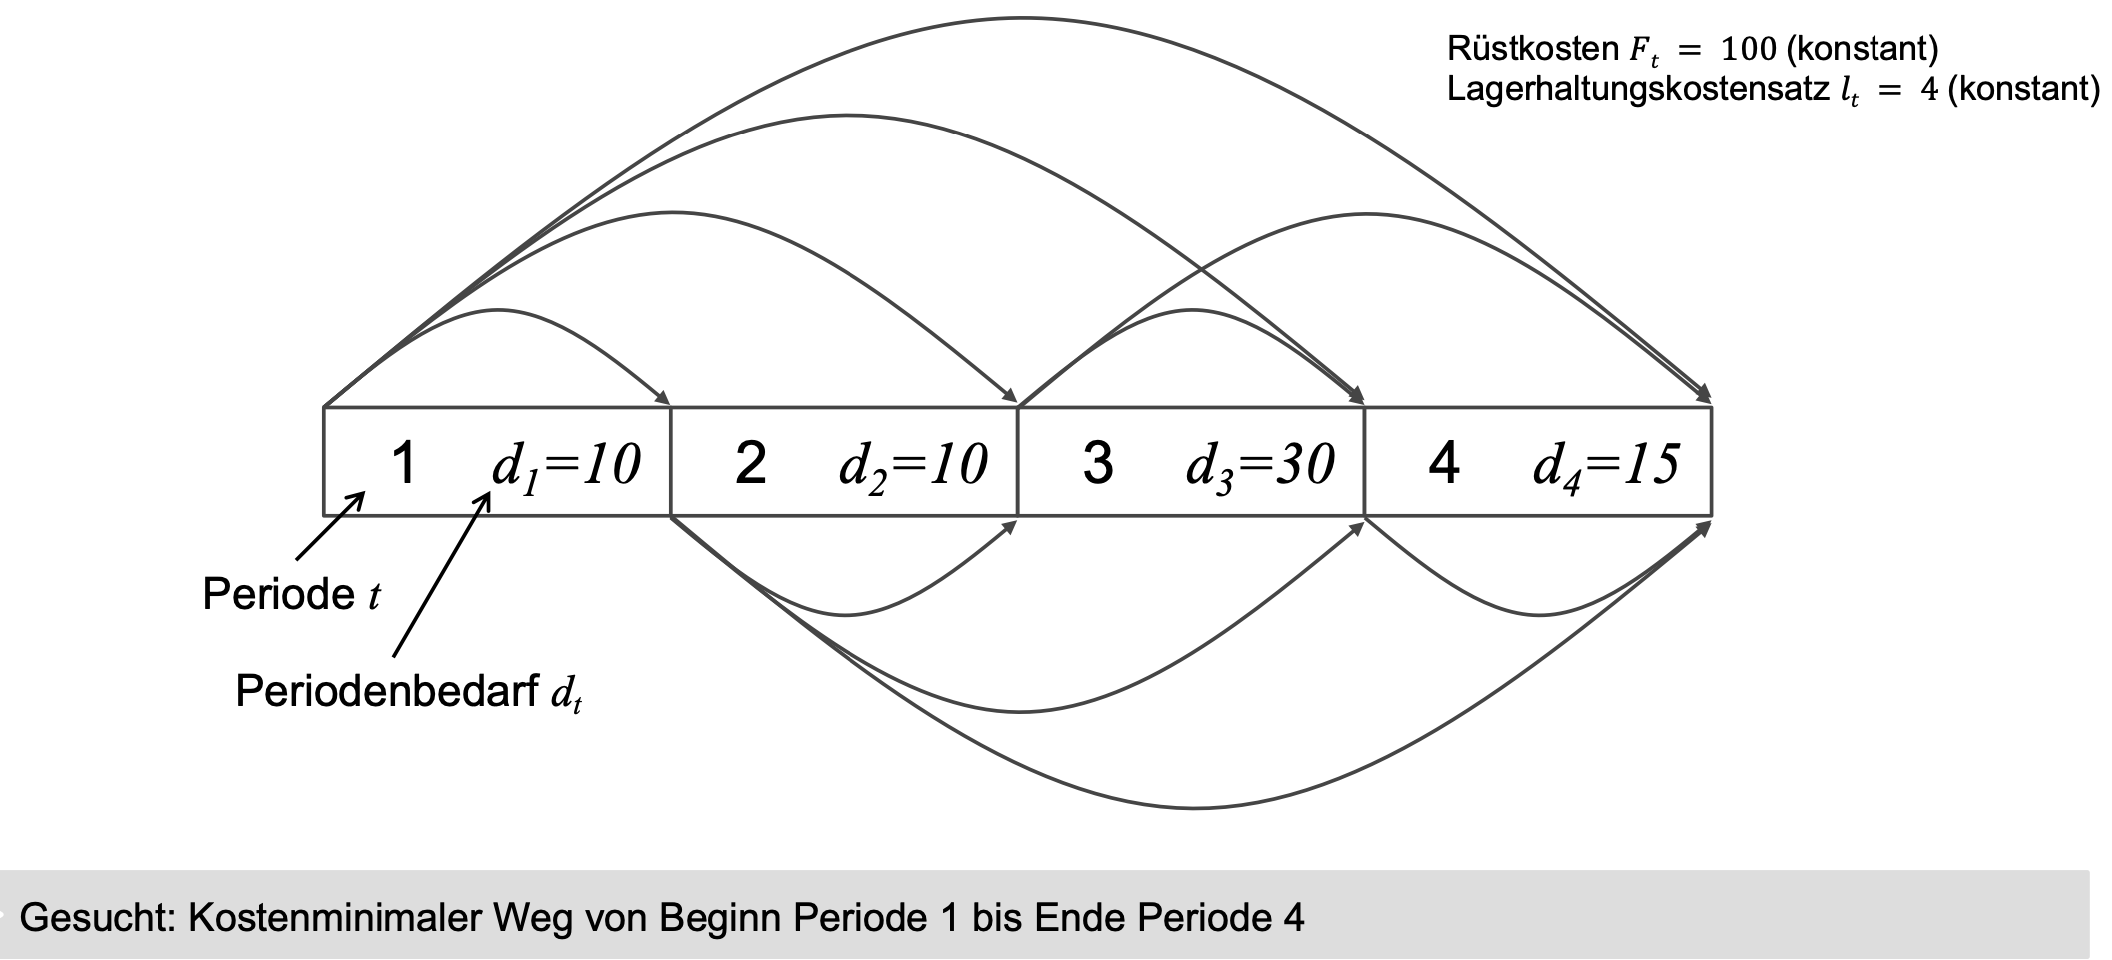
\includegraphics[width=0.6\linewidth]{VL81.png}
\end{figure}




\newpage
\item Funktion
\begin{enumerate}


\item ZF:

\begin{center}
$min Z = f_k$\\
minimale Wegkosten
\end{center}

\item u.d.N

\begin{center}
$f_k = min\{f_{t-1}+c_{tk}\}$\\
$f_0=0$
\end{center}

\item 满足Deckung\\
\begin{center}
$c_{tk} = F_t + l_t \cdot \sum_{v=t+1}^{k}(v-t) \cdot d_v$\\
自身的Fix (Rüste) +\ Kostensatz$\cdot$覆盖周期
\end{center}

\item $p_k = f_k$

\end{enumerate}




\end{itemize}


%%%%%%%%%%%%%%%%

\newpage
\section{Losgrößenplanung – Teil 2}

\subsection {Mehrstufige kapazitierte Losgrößenplanung in der Werkstattproduktion}
\begin{itemize}
\item Methoden der Losgrößenplanung:\\[1mm]
\textbf{simultane Planung} - Mehrstufige kaprizieret Losgrößenplanung\\
同时规划 - 多级容量约束的批量规划

\item Modell MLCLSP \textbf{\textcolor{red}{(针对生产时间)}}\\
Ergebnis: Bestimmung der prinzipiellen Maschinenrüstung, der Produktionslose sowie der Lagerbestände\\
Ziel: Summer der \textcolor{blue}{Kosten (Lager- und Rüstkosten) minimieren}\\[1mm]
\textcolor{green}{Vorteil}: 顾及了Struktur- und zeitliche Zusammenhänge von Erzeugnissen


\item Funktion:\\

\begin{enumerate}


\item ZF:
\begin{center}
$min Z = \sum_{tjk}^{TJK} \textcolor{red}{F_{jkt} \cdot \gamma_{jkt}}
 +\sum_{tk}^{TK} \textcolor{orange}{ l_k \cdot L_{kt}}$\\
 产品k\ 周期t\ 资源j\\
\textcolor{red}{Rüstkostensatz\ 1/0} + \textcolor{orange}{Lagersatz\ Bestand}
\end{center}

\item 内存限制 (Anzahl: JT):
\begin{center}
$\sum_k (tb_{jk} \cdot q_{jkt} + tr_{jk} \cdot \gamma_{jkt}) \leq c_{jt}$\\
 单个加工时间 $\cdot$ 产生的Los + Rüstzeit $\cdot$ 1/0\\
 \end{center}
 
 \item Bilanz (Anzahl: KT):
\begin{center}
$\L_{kt} = L_{k,t-1} + \sum_j q_{j,k,t-z_k}
- \sum_i a_{ki} \cdot \sum_j q_{jit} - d_{kt}$\\
 = 上周期剩余+之前Los之和-系数$\cdot$现在Los之和-需求\\
 \end{center}


\end{enumerate}
\end{itemize}

\newpage
\subsection{Losgrößenplanung in der Fließproduktion (Einproduktfall) 单一产品在一流水线}


\begin{itemize}


\item Fließproduktionslinie 流水线的优缺点\\[1mm]
V: sehr hohe Auslastung\\[1mm]
N: geringe Flexibilität

\item Ziel: Bestimmung der kostenminimalen Losgröße


\item Funktion:

\begin{enumerate}

\item ZF:
\begin{center}
$Min C = \frac{d}{q} R + \frac{l}{2}[q(1-\frac{d}{p})]$\\
单位时间平均成本最小化
\end{center}


\item optimale Losgröße 

\begin{center}
$q^* = \sqrt{\frac{2\cdot\ d \cdot R}{l \cdot (1-\frac{d}{p})}}$\\
d: 消耗率 \ p: 生产率\\ R: Rüstkosten\ l: Lagerkosten
\end{center}

\item 最大库存
\begin{center}
$L = q^*(1-\frac{d}{p})$\\
\end{center}


\item 生产时间
\begin{center}
$t_p = \frac{q^*}{p}$\\
\end{center}

\item 循环时间
\begin{center}
$Z = \frac{q^*}{d}$\\
\end{center}

\end{enumerate}

\end{itemize}



\newpage
\subsection{Losgrößenplanung in der Fließproduktion (Mehrproduktfall) 多种产品在一流水线}

\begin{itemize}

\item Herausforderung
\begin{enumerate}
\item Verfügbarkeit der Produktionsanlage von 100\% ist nicht realistisch
\item Erweiterung um reihenfolgeabhängige Rüstzeiten
\item Berücksichtigung von mehreren Produktionsstufen

\end{enumerate}


\item Funktion

\begin{enumerate}

\item 理想生产循环时长
\begin{center}
$T_{opt}=\sqrt{\frac{2\sum_kR_k}{\sum_k [d_k \cdot l_k(1-\frac{d_k}{p_k})]}}  $
\end{center}


\item 循环时长下限 \textcolor{blue}{untere Schranke}
\begin{center}
$T_{min}=\frac{\sum_k \tau_k}{1-\sum_k\frac{d_k}{p_k}} \leq T_{opt}$
\end{center}


\item 理想Losmenge
\begin{center}
$q_k=d_k\cdot T_{opt}$
\end{center}


\item Belegungszeit 繁忙时间
\begin{center}
$t_{ges}=\sum_k \tau_k + (\frac{q_k}{p_k})$
\end{center}


\end{enumerate}

\end{itemize}



\end{CJK*}
\end{document}
